\chapter{On Algorithms for Building and Sampling Disordered Crystal States}
\label{ch:iceXI}

\section{States and Properties of Ice}

%Ice has many forms, each with unique environments and structures that give rise to similar and distinct properties. 

\subsection{Bernal-Fowler Ice Rules}

First described in John Desmond Bernal and Ralph H. Fowler's 1933 paper, the Bernal-Fowler Ice Rules are the foundational observations of how water molecules interact in an ice structure.\cite{BFIceOG}
Although a bent, divalent molecule, water possesses an electronic tetrahedral structure that allows for four interactions on each molecule.
The two protons each allow for a hydrogen bond with a lone pair from a neighboring oxygen atom.
Similarly, the oxygen atom's two lone pairs each allow for a hydrogen bond with a neighboring proton. 
While a hydrogen bond is typically defined as an attractive interaction between a proton and one lone pair of electrons on Nitrogen, Oxygen, or Fluorine, this work restricts the definition to a computational implication.
Here, a hydrogen bond refers to the space between two oxygen atoms in a crystal where exactly one proton and lone pair are directed toward one another according to Bernal-Fowler ice rules. 
Fortunately, this difference is sufficiently small for visualization programs like Avogadro to still recognize hydrogen bonds between a rotated hydrogen atom and corresponding neighboring lone pair. 
These rules are fairly rigid in the sense that every water molecule can interact with two oxygen atoms and two protons from four surrounding water molecules.
These are also relatively relaxed in the sense that, once hydrogen bonded, each of the four attached water molecules can occupy one of three rotational positions. 
Including the 6 orientations of the central water, 486 microstates exist from these five waters.

\subsection{Forms of Ice}

While ubiquitous in the `I$_{h}$' form, ice water has many phases.
As of the writing of this work, there are 18 experimentally established forms of ice. 
These forms usually occur in cubic, hexagonal, and orthorhombic crystal structures.
As can be seen in figure \ref{fig:icePhases}, the system pressure and temperature are primary characteristics of which phase will form.
The subject of this work will be on the proton-ordered orthorhombic ice XI and its proton-disordered isomer, ice I$_{h}$.

\begin{figure}
	
	\centering
	
	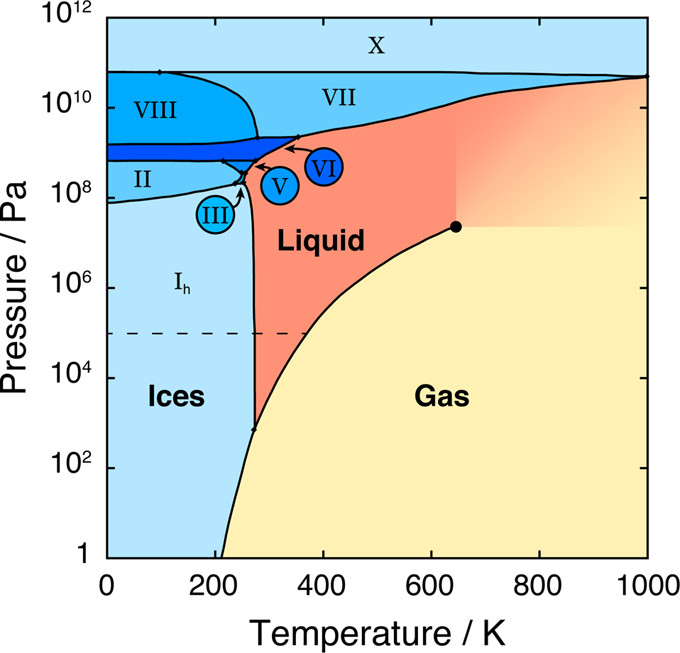
\includegraphics[width=0.75\textwidth]{icephase.jpeg}
	
	\caption{Water phase diagram. Taken from Brini et al. \cite{BriniWaterProperties}}
	
	\label{fig:icePhases}
	
\end{figure}

\subsection{Ice I$_{h}$}

Ice I$_{h}$ naturally forms at temperatures below 273.15 K at pressures in the 1 Pa to 100 MPa range,\cite{IceTPLimits} with some temperature curving off into the vapour and liquid phases at very high and very low pressures as seen in figure \ref{fig:icePhases}.
As the most commonly found form on earth, ice I$_{h}$ is the most relevant form for computational studies involving ice systems.

As famously discussed by Linus Pauling, hexagonal ice water contains a residual entropy at very low temperatures.\cite{PaulingIce} 
This residual entropy in ice goes according to Boltzmann's entropy equation $S=K_{B}LnW$ where $W=(\frac{3}{2})^{N}$ for $N$ molecules in the crystal.
At near absolute zero temperatures, the residual entropy will not reach zero as the disordered water could settle into one of many microstates that fit the ``disordered" description.
Pauling additionally predicted that an ice structure with perfectly ordered protons may exist at sufficiently low temperatures with zero residual entropy.
% WHY IS ICE IH MORE VALUABLE IN RESEARCH???????
% As an interesting specificity, the ice I$_{h}$ structure does not include any proton-disordered crystal with the same oxygen spatial positioning. % NEED SOURCE BEFORE INCLUDING

%% REMOVED: REDUNDAND WITH LATER SECTION
%\subsection{Efforts to Generate Ice I$_{h}$}
%
%
%A commonly referenced effort to create an ice I$_{h}$ crystal comes from Victoria Buch's 1998 paper. \cite{MCIce}
%Her work involved a Monte Carlo effort to generate ice I$_{h}$ by initializing a deprotonated oxygen structure, randomly placing the appropriate number of protons, and then using MC methods to adjust the structure until every oxygen atom was bonded to exactly two protons according to Bernal-Fowler ice rules.


\subsection{Comparison between Ice XI and Ice I$_{h}$}

While ice I$_{h}$ is known as the most common form of ice found on the planet, it is much more difficult to computationally generate than an ice XI crystal. 
The ease of generation of an ice XI structure stems from the repetition of a unit cell with consistent layering and orientation throughout the crystal lattice. 


With ice I$_{h}$ crystals, the proton-disordered form introduces entropy by way of rotational disorder of water molecules. 
The disordered protons allow for a greater number of microstates in the organization of the crystal, increasing the multiplicity and, by its very definition, entropy.
As the protons and lone pairs are no longer consistently ordered, hydrogen bonds may no longer form properly at all interaction sites. 
Fortunately, this difference is sufficiently small for visualization programs like Avogadro to still recognize hydrogen bonds between a rotated hydrogen atom and corresponding neighboring lone pair. 
The interaction of proton with proton or lone pair with lone pair are not hydrogen bonds and are considered defects in the lattice. 
These are known as Bjerrum defects and referred as D with two protons or L with two lone pairs interacting.\cite{BjerrumDefects}
Conversely, hydrogen bonding does not occur if Bjerrum L or D defects occur between the oxygens.
An ice structure of randomly oriented molecules without consideration of hydrogen bonds will likely produce defects at many interaction sites across the lattice and weaken the integrity of the crystal, leading to stability problems while running simulations. 
In generating the crystal, the cause of these defects must be considered and countered effectively.
While other stable hydrogen bonding structures may exist, they would either break the Bernal-Fowler ice rules or alter the structure away from the specified form.



\section{Method Design}

% overview
% 0. get pdb ice xi DONE
% 1. read in pdb ice xi DONE
% 2. identify molecules (H2O) DONE 
% 3. identify molecule neighbors DONE
% 4. identify corners/edges (in progress) DONE
% 5. for each molecule, identify the tetrahedral spaces DONE
% 6. for each molecule, "randomly" place the two protons DONE
% 7. Check hydrogen bond defect rate DONE
% 8. Fix as necessary (in progress) DONE
% 9. Compare to existing work

\subsection{Method Tools and Information Management}

The primary objective is to convert an easy-to-make ice XI crystal into an ice I$_{h}$ crystal.
Because the key difference in structure is the proton-orderedness, it might be possible to rearrange the water molecule orientations in a pseudorandom way to create an ice I$_{h}$ crystal.
This section walks through the method developed to convert ice XI into ice I$_{h}$, the results of initial testing, and imperfections discovered in the design.

%\subsection{Selection of Software Tools}

Python was chosen as the programming language of the tool due to its versatility and the ease of development due to the ``pseudocode" written style and the availability of scientific packages including SciPy and NumPy. 
Python version 2.7 was specifically utilized.
Crystal files where defined and saved as Protein Data Bank (.pdb) files as this format allows for defining multiple molecules within a larger structure with a simple X, Y, Z grid position format. 
An example of this is provided in Appendix \ref{ch:App:CrystalDisorg}.

%\subsection{Generation of Source Ice XI}

To create an ice XI .pdb file, an ice XI cell of eight water molecules can be tiled to create a sufficiently large crystal.
The primarily used crystal consists of a 3 x 3 x 6 cell repetition totaling 432 water molecules.

%\subsection{Source Ingestion}

It is important that the crystal be read and stored in an efficient method to keep relevant information about each molecule easily accessible. 
As the file is read in, each molecule is stored as an entry in a multidimensional array where the first index is the molecule number. 
Further, the second index defines the molecule number where 0 is oxygen and 1 and 2 are the protons. 
The third, fourth, and fifth indices define the X, Y, and Z position coordinates. 
This is functionally identitical to the .pdb format data, but compresses the data across multidimensional arrays for iterative use.

%\subsection{Identifying Neighboring Molecules}

Identifying the neighboring molecules proved computationally difficult. 
The most effective method is to find the closest four molecules by computing a distance between every two oxygen atoms.
This ensures every molecule is considered, but also presents significant hurdles.
First, a distance calculation utilizes a computationally-inefficient square root calculation.
The inefficiency lies in the binary-based command for calculating a square root that often utilizes either a logarithmic solution or a Newtonian approximation that typically requires 16-64 processor cycles.
This square root computation can be entirely bypassed by instead comparing the squared-distance between molecules and finding the lowest values.
These squared-distances scale identically to the square root value for all distances greater than one, which is true for the ice XI structures sampled in this work.

Second, molecules positioned along the sides  will not have four neighbors in a non-periodic crystal. 
This is accounted for by shifting all six sides to make a pseudo-periodicity for these edge cases. 
Those periodically-neighboring molecules are flagged with a shifting value in the neighboring atom array by specifying a translation in the x, y, or z axis values. 
%% it can be done easily.
%Unfortunately, the necessary code to implement the periodically-neighboring molecule detections requires a major rewrite of the entire tool and has not yet been implemented.

Once these four neighboring oxygen atoms have been discovered for each water, the four hydrogen-bond interactions according for Bernal-Fowler ice rules with the neighbors describe an orientation defined by the location of each water's protons and lone pairs located at coordinates called tetrahedral positions.
%Once these closest neighboring oxygen atoms have been discovered, the appropriate interacting tetrahedral position is identified by finding the closest of the four tetrahedral positions using the same squared-distance calculation with the four defined tetrahedral positions detailed in the next subsection.


% NEEDS SIGNIFICANT WORK
%\subsection{Determining Tetrahedral Positions}

An important aspect of pseudorandom selection is the existence of a bank of options.
Utilizing the ingestion portion of the tool to calculate and store all orientational possibilities proves effective for tracking position options.
In this work, tetrahedral positions are defined as the four positions that a proton may occupy about a water molecule as the four electron groups extend from the oxygen.
For each water molecule, the first two tetrahedral positions are defined by the positions of the two hydrogen atoms. 
The other two positions are found by rotating one hydrogen atom 120$^{\circ}$ twice about the vector from the oxygen atom through the other hydrogen atom and storing the resulting positions as tetrahedral positions three and four. 
Prior to rotation, the third and fourth positions are occupied by lone pairs.
According to the .pdb file style, though, lone pairs are implied from the atom data and are not explicitly stated in the file data.
This allows for passive relocation of the lone pairs by redefining the proton positions about the water.
A visualization of these four tetrahedral positions, two read and two generated, are shown and labeled in figure \ref{fig:tetXI}.

\begin{figure}
	
	\centering
	
	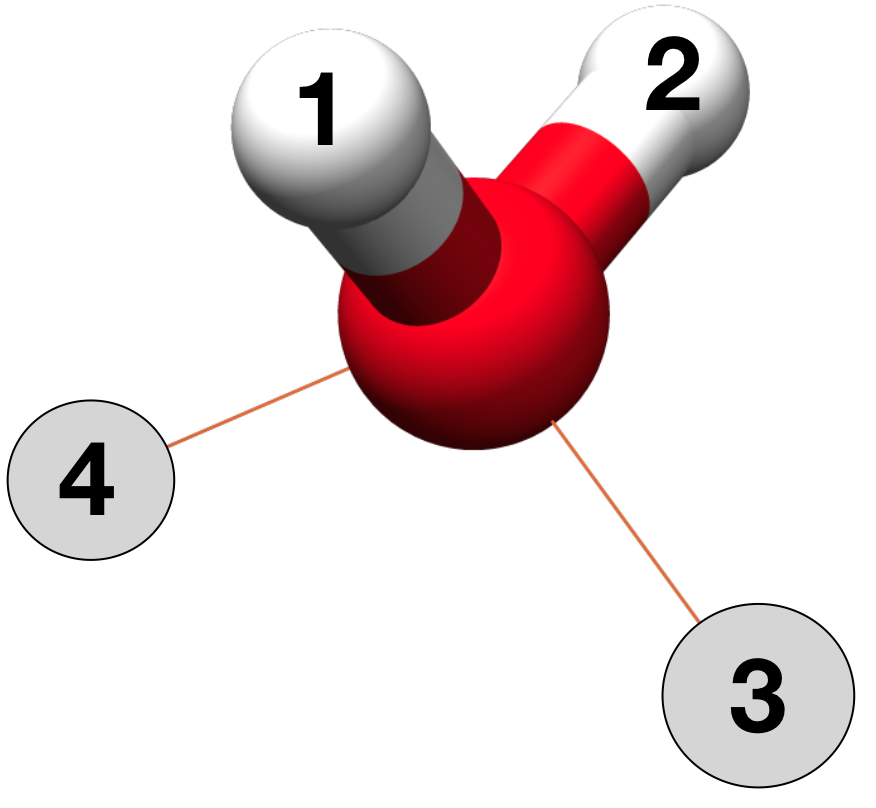
\includegraphics[width=0.6\textwidth]{tetIce.png}
	
	\caption{Example Tetrahedral positions of a water molecule. The two spheres represent potential proton positions roughly occupied by lone pairs.}
	
	\label{fig:tetXI}
	
\end{figure}

% something about normal 109.5º tetrahedral angle
In a equally-repulsed tetrahedral molecule, electron group angles are 109.5$^{\circ}$.
This method does not produce an exactly correct tetrahedral position of potential hydrogen atoms due to the slightly acute104.5$^{\circ}$ H-O-H bond created by the variance in repulsive forces between the two lone pairs of electrons and two hydrogen atoms.
Fortunately, this difference is sufficiently small for visualization programs like Avogadro to still recognize hydrogen bonds between a rotated hydrogen atom and corresponding neighboring lone pair. 
Currently, the method does not correct for these minor angle variations and relies on the user to anneal the crystal by way of simulation to fully adjust the angles. 
Future versions of this method may account for the variations.

\subsection{Pseudorandom Rearrangement of Water Molecules and Generation of Bjerrum Defects}

Once the tetrahedral positions have been defined, each water molecule is ready to rotate.
What may seem the most crucial step in this methods ends up being the most simple.
%As designed, the rotation of water molecules is as simple as using a stepwise iterator to pseudorandomly select two tetrahedral positions for the hydrogen bonds and store the new positions in a new crystal array. % REVIEW
The act of rotating each proton about the corresponding oxygen atom in a crystal is as simple as iterating through and pseudorandomly selecting two tetrahedral positions from each water for protons to occupy.
The new position data is saved to a new crystal array file similar to the parent generated during the initial file read.
These new positions are determined sequentially and ``instantaneously" in the time-independent manipulation of the crystal.
An important note is that this rearrangement does not consider the orientations of neighboring molecules and likely introduces Bjerrum defects.
The likelihood of a defect-free interaction lattice forming is nearly zero and is presumed to have a large number of defects within the lattice. 
For example, the first molecule reoriented will have a $\frac{5}{6}$ chance of containing a defect.


%\subsection{Detecting Hydrogen Bond Defects}

After all water molecules have been rearranged, defects between incorrectly-interacting hydrogen bonds must be found and corrected.
Discovering the defects relies on the detection of neighboring molecules and the appropriate interacting hydrogen atom or electron lone pair. 
As previously discussed, the initial data ingest records and detects the nearest water molecules and determines the tetrahedral position containing the interacting space, be it electron lone pair or hydrogen atom. 
From that data, the detection of a valid hydrogen bond is as simple as checking both interacting tetrahedral positions between two neighboring waters and confirming that they do not both contain or lack a hydrogen atom.
Each water maintains a count of how many defects are present among the four positions, which can be collectively averaged for a per-molecule defect average.
Likewise, these defects can be summed and halved to produce a total number of defects in the crystal. 
Each molecule holding its own defect count allows for contextual changes during the correction step.


%\subsection{Correcting Hydrogen Bond Defects}

Once the hydrogen bond defects have been discovered and marked, each needs to be corrected.
The most direct approach to this is to sequentially walk through each defect and repeat the pseudorandom rotation until the number of defective regions is zero or a user-specified value.
The current implementation sorts the defect list by the number of defects and attempts to fix the most defective molecules first because of the highest-density entropy introduced into the system.
These most defective molecules may include defects impossible to solve by simple rotation, specifically when neighboring molecules have collectively directed three or four hydrogen atoms or electron lone pairs at the target water. 
These can only be solved by adjusting one or more of the neighboring molecules until the number of hydrogen atoms and electron lone pairs have balanced.
Unfortunately, this high-defect problem can quickly escalate if the neighboring molecules contain the same problem of unbalanced hydrogen atoms and electron lone pairs. 
The current solution is to recursively check for and fix these impossible interactions first, but has not yet yielded a defect-free crystal in testing.

The current design of the method allows for the user to specify a threshold of defects as an average per molecule. 
For example, a threshold of 2.5 will allow a maximum of 3 defects on any given molecule and will continue to correct defects until the average number of defects per molecule is equal to or below 2.5.
Because each of these defects will be counted twice, once for each molecule, the total number of defects in a crystal can be determined by multiplying the average defect value by the number of molecules and dividing by two.
As of the current implementation, the method cannot reliably produce a crystal with a threshold below 2 as it will continue to recursively search until the system runs out of available memory and crashes without finalizing the structure.
The memory overflow is due to the infinite recursion instead of repeatedly storing new crystal data.

\section{Results of Method}

When supplied with an input ice XI crystal, an output structure with rotated water molecule orientations strictly consistent with ice I$_{h}$ describes a success at the most basic level.
An example before and after of the method is given in figures \ref{fig:iceXI} and \ref{fig:iceIh}.
\begin{figure}
	
	\centering
	
	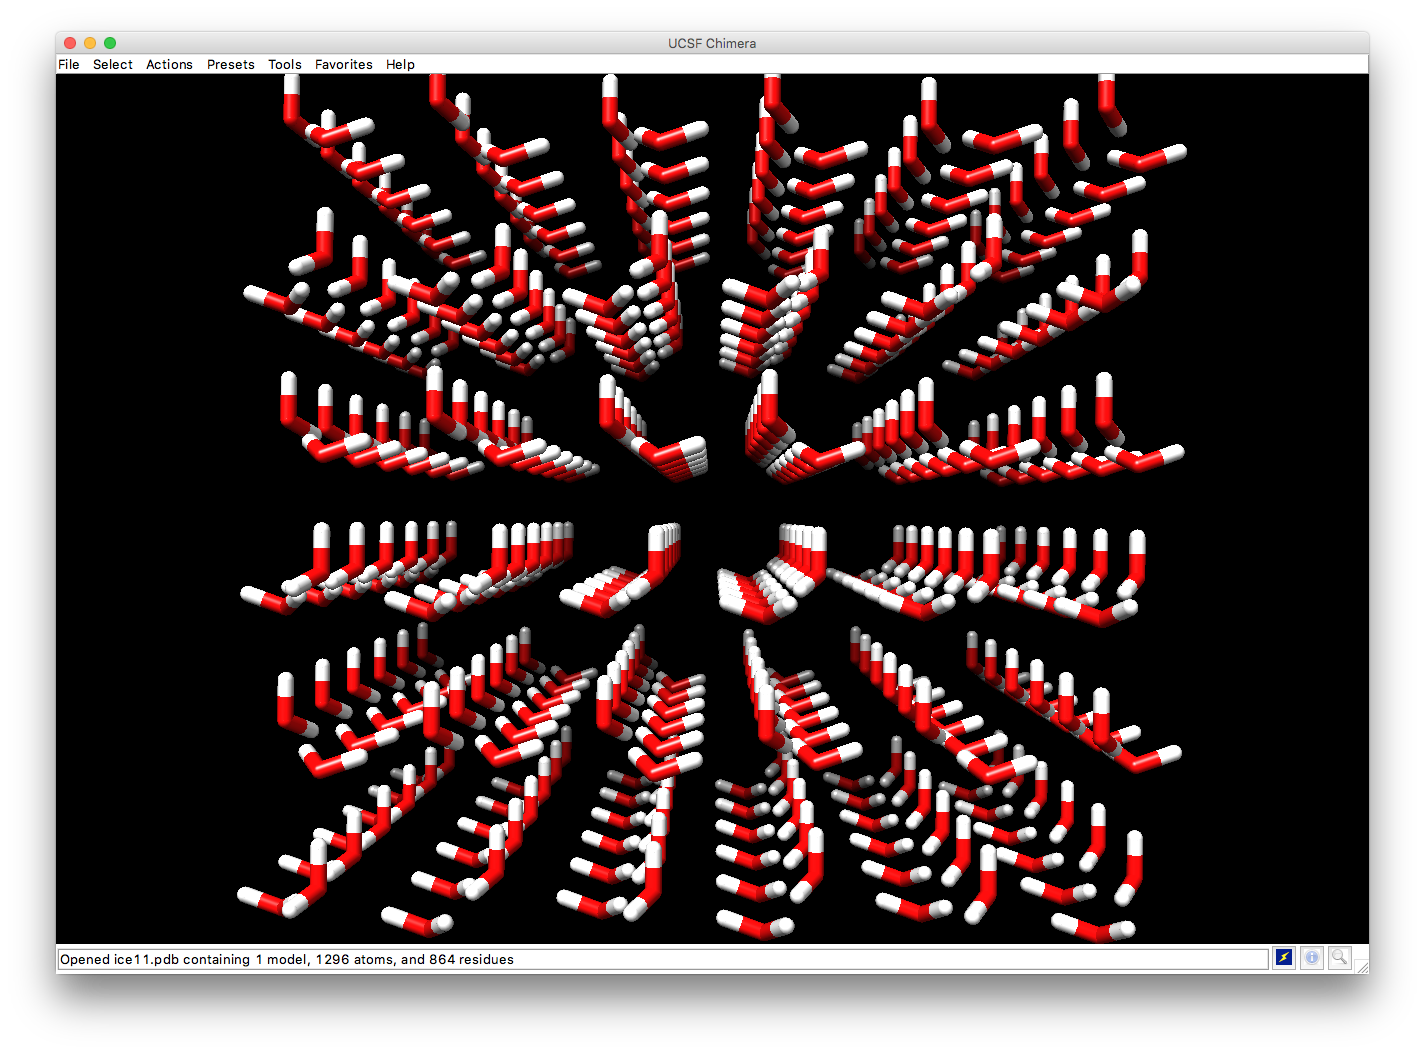
\includegraphics[width=0.75\textwidth]{iceXI.png}
	
	\caption{``Before" image of Ice XI}
	
	\label{fig:iceXI}
	
\end{figure}
\begin{figure}
	
	\centering
	
	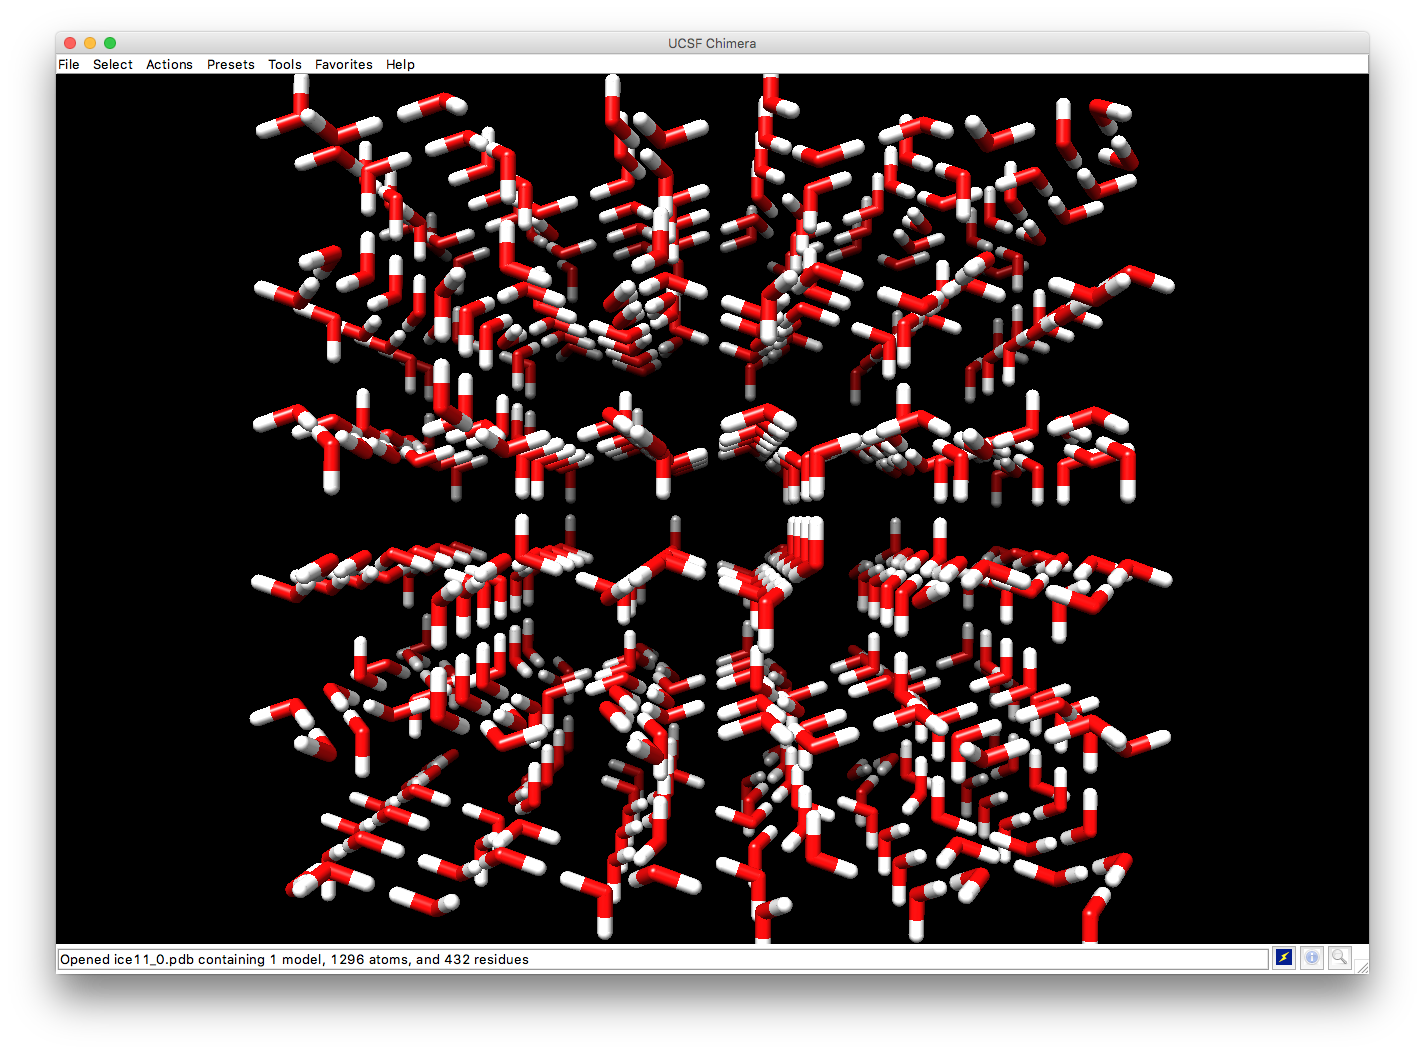
\includegraphics[width=0.75\textwidth]{iceIh.png}
	
	\caption{``After" image of generated ice I$_{h}$}
	
	\label{fig:iceIh}
	
\end{figure}
As can be seen, the ``after" image has experienced rotation and can no longer be classified as ice XI. 
%However, as ice I$_{\mathrm{h}}$ also has a standard shape, the generated crystal can not be considered ice I$_{\mathrm{h}}$.
Instead, it can be considered a proton-disordered orthorhombic ice crystal similar to ice I$_{h}$. 

Unfortunately, the result is not without defect.
When following the subsequent layers in the crystal, patterns emerge. 
Inconsistently, some rows of waters remain consistent.
Some of these are a uniform rotation of both hydrogen atoms consistent across rows.
These consistent rows can be observed in figure \ref{fig:iceIh} toward the center-left and center-right along the into-the-page axis.
Multiple trials yield internally unique results, yet all contain these strange consistencies.
This may be due to some accidental pattern in the method's implementation.
A scoring function to analyze the ``randomness" of the crystal would confirm whether this pattern is imagined or real.

% FINISH
%
%
%
%
\section{Comparison to Buch's Method}

In her 1998 paper, Victoria Buch proposed a MC-based system for converting ice XI to ice I$_{h}$.\cite{MCIce} 
In that method, an ice XI crystal would have all protons dissociated from oxygens by moving them to halfway between corresponding oxygens.
By placing protons in the middle of two oxygens, this allowed MC methods to pseudorandomly move the protons toward one or another oxygen.
Once moved, the Bernal-Fowler rules are applied to increase the chance of a proton association switch being accepted for invalid waters.

As a comparison to this work, Buch's method is more likely to successfully produce a defect-free ice I$_{h}$ crystal.
In its current state, this work's method is not as efficient nor as effective as Buch's method.
As a potential for future development, this method allows for defects to exist as a state value which could be used for annealing studies.



\section{Comments on Limitations and Proposed Improvements}

During the hydrogen bond defect correction step, a weakness in the design is that any clustering or regions of high defect density will not be treated uniquely.
This allows the existence of a highly-defective region within the larger structure that could potentially cause problems when the crystal is used in simulations. 
The prevalence and occurrence of these defects have not been studied in this work, but seem a natural inevitability of statistics. 
% SHOW THE STATS
A potential solution with partial development will score regions based on the number of defects as a weighted function expanding out from a central molecule for $N$ connections. 

For example, consider a specific water defined as level 1. 
The neighboring four molecules are defined as level 2, and continued onward excepting already-defined molecules out to an $N^{th}$ level. 
No special considerations for waters with fewer than four neighbors are necessary as periodic generation would allow ``edge" waters to interact with the periodic continuation waters.
The number of defects in each level can be counted and averaged.
Then a depressive factor along the lines of $\frac{1}{level}$ can be used to diminish the value of defects further away from the first-level molecule.
This would create a value for each molecule that shows the relative density of defects centered about that specific molecule and could even be plotted as a gradient change within the crystal.
The general approach to a scoring mechanism may take a form similar to equation \ref{eq:IceScoring}.
If effective, a scoring function like below would build a better queue for the defect correction step in an MC fashion as it works toward identifying and reducing the defect density.
\begin{equation}
\label{eq:IceScoring}
Value = \sum_{l=1}^{N_{levels}} \Big[\frac{1}{l} * \frac{1} {N_{molecules}} *\sum_{m=1}^{N_{molecules}}[N_{defects, m}]\Big]
\end{equation}

%final thoughts?




